\documentclass[12pt]{article}
\usepackage{url,graphicx,tabularx,array,geometry}
\usepackage{listings}
\usepackage[utf8]{inputenc}
\usepackage{setspace}
\usepackage{amsmath}
\usepackage{enumitem}
\setlength{\parskip}{1ex} %--skip lines between paragraphs
\setlength{\parindent}{0pt} %--don't indent paragraphs

%-- Commands for header
\renewcommand{\title}[1]{\textbf{#1}\\}
\renewcommand{\line}{\begin{tabularx}{\textwidth}{X>{\raggedleft}X}\hline\\\end{tabularx}\\[-0.5cm]}
\newcommand{\leftright}[2]{\begin{tabularx}{\textwidth}{X>{\raggedleft}X}#1%
& #2\\\end{tabularx}\\[-0.5cm]}

\onehalfspacing
%\linespread{2} %-- Uncomment for Double Space
\begin{document}

\title{Imperative and System Programming Autumn 2013}
\line
\leftright{\today}{Alexander Rüedlinger, 08-129-710} %-- left and right positions in the header
\section*{Series 2}
\subsection*{Part 1: C}
\paragraph{Remarks}
\begin{itemize}[noitemsep]
\item ASCII is a character-encoding scheme that encodes 128 specified characters. The ASCII code is the numerical representation of characters.
\item In the ASCII table the integer value 65 corresponds to the character 'A'.
\item The character '@' corresponds to the value 64.
\end{itemize}

\subsubsection*{1. Type Conversion, Casting and ASCII Table}
\begin{lstlisting}
(1) printf("%c %i\n", c, c);
\end{lstlisting}

The format specifier \%c and \%i are substitued with the matching argument in the printf argument list. 
So the specifier \%c will be replaced by the second argument c and the specifier \%i by the third argument c. The specifier \%i converts the third argument (char value) to an integer.

The statement (1) prints:\\
A 65
\\
\begin{lstlisting}
(2) printf("%c %i\n", i, i);
\end{lstlisting}
In the statement (2) the first format specifier \%c converts the int value i to a char 'A'. The second format specifier replaces the value without a conversion, because the veriable is already an integer.
The output is given by:\\
A 65
\\
\begin{lstlisting}
(3) printf("%f %i\n", pi, (int)pi);
\end{lstlisting}
The first format specifier takes a variable of type float and the second one a variable of type int.
Because the third argument in printf() is explicitly casted to an integer, the variable pi is truncated, so it's floating point part is lost. Thus the printf statement above prints:

3.14 3

\subsubsection*{2. Constant, Variable, Escape Character '\textbackslash', and Octal resp. Hexadecimal Digits}
\begin{lstlisting}
(0) #define AT '\100'
\end{lstlisting}
The line above creates a symbolic constant with the content '\textbackslash 100'.
Every occurrence of the symbolic constant AT will be substituted with '\textbackslash 100' by the C preprocessor.

\begin{lstlisting}
(1) char at = '\x40'; // variable in hexadecimal
\end{lstlisting}
This line creates a char variable using an hexadecimal constant. The hexadecimal value is equals to 64 in the decimal number system.
\begin{equation}
\text{at} = [4 \: 0]_{16} = [0100 \: 0000]_2 =  [64]_{10}
\end{equation} 
Because character values are internal stored as integers the ASCII value 64 corresponds to the @ symbol.
\\
\begin{lstlisting}
(2) printf("%c %i %o %x\n", '@', '@', '@', '@');
\end{lstlisting}
The printf statement uses four different format specifiers for the character @.
The \%c specifier is substituted by the character @. The other specifiers \%i, \%o and \%x convert the char '@' to an integer, octal and hex value. 
A computation for each number system yields:
\begin{equation}
\begin{split}
@_{char} = {[64]}_{10} = {[2^6]}_{10} = {[0100 \: 0000]}_2 \\
= [1 \: 0 \: 0]_{8} =[4 \: 0]_{16}
\end{split}
\end{equation}

So the output of this printf statement is given by:

\begin{lstlisting}
@ 64  100 40
\end{lstlisting}


\begin{lstlisting}
(3) printf("%c %i %o %x\n", AT, AT, AT, AT);
\end{lstlisting}
Each of the symbolic constants AT is replaced by the octal constant '\textbackslash 100'. The format specifiers given in the printf statement convert the octal value $100$ to a char (\%c), int (\%i), octal (\%o) and hex value (\%x). 
The output is as follows:
\begin{lstlisting}
@ 64  100 40
\end{lstlisting}


\begin{lstlisting}
(4) printf("%c %i %o %x\n", at, at, at, at);
\end{lstlisting}
In the line above a hex constant '\textbackslash x40' is converted according the specified format specifiers. Firt specifier converts the hex value to char, the second one to int, the third one to octal and the last one to hex. 

This yields the output:
\begin{lstlisting}
@ 64  100 40
\end{lstlisting}


\subsubsection*{3. enum Type}
\begin{lstlisting}
(0) enum {FALSE, TRUE} b; // declaration of variable b,
                          // without tag
\end{lstlisting}
This line declares the enum values FALSE and TRUE but without a tag. In ANSI C, an enum constant is always of type int. So internal they're represented by the integers 0 (FALSE) and 1 (TRUE). The ordering in the enum construct specifies the internal integer representation. By default the first enum value in the enumeration is associated with value zero. Besides that the veriable b of enum type TRUE is declared.
\\
\begin{lstlisting}
(3) printf("%i %i\n", b, FALSE);
\end{lstlisting}
Because the variable b and the enum type FALSE is internal stored as an integer no conversion is necessary. So the format specifiers are just substituted by the integer values.

Output:
\begin{lstlisting}
1 0
\end{lstlisting}

\begin{lstlisting}
(4) enum color_tag {RED, GREEN, BLUE};
\end{lstlisting}

Here we declare an enum with tag color\_tag . As mentioned before, each of these enum values are represented by ints, so we have RED=0, GREEN=0 and BLUE=2.
\\
\begin{lstlisting}
(7) c1 = RED; c2 = c1+1; c3 = BLUE;
\end{lstlisting}
In the line above the variables c1, c2 and c3 are initialized with values c1=0, c2=1 and c3=3. In this example we use the fact that integer arithmetic operations can be performed on enum values.

Therefore, the printf statement (8) produces the output:
\begin{lstlisting}
0 1 2
\end{lstlisting}
\newpage
\subsubsection*{4. Logical Expressions}
\begin{table}[!htb]
\centering
\begin{tabular}{|c|c|c|c|}
\hline
$p$ & $q$ & $!q$ & $ p \quad || \quad !q$ \\ \hline \hline
t & t & f & t \\ \hline
t & f & t & t \\ \hline
f & t & f & f \\ \hline
f & f & t & t \\ \hline
\end{tabular}
\caption{Logical expression 1}
\end{table}

\begin{table}[!htb]
\centering
\begin{tabular}{|c|c|c|c|}
\hline
$p$ & $q$ & $(p==q)$ & $ p \quad \&\& \quad (p==q)$ \\ \hline \hline
t & t & t & t \\ \hline
t & f & f & f \\ \hline
f & t & f & f \\ \hline
f & f & t & f \\ \hline
\end{tabular}
\caption{Logical expression  2}
\end{table}

\begin{table}[!htb]
\centering
\begin{tabular}{|c|c|c|c|c|c|}
\hline
$p$ & $q$ & $(p=q)$ & $(p=!q)$ & $p \quad \&\& \quad (p=q)$ & $(p \quad \&\& \quad (p=q)) \quad || \quad (p = !q)$\\ \hline \hline
t & t & t & f & t & t\\ \hline
t & f & f & t & f & t \\ \hline
f & t & t & f & f & f \\ \hline
f & f & f & t & f & t\\ \hline
\end{tabular}
\caption{Logical expression  3}
\end{table}
\newpage
The C compiler evaluates the logical expression from left to right:
\begin{lstlisting}
(2) p && (p=q) || (p = !q)
\end{lstlisting}

The expression above can be represented by the following abstract syntax tree:
\begin{figure}[!htb]
\centering
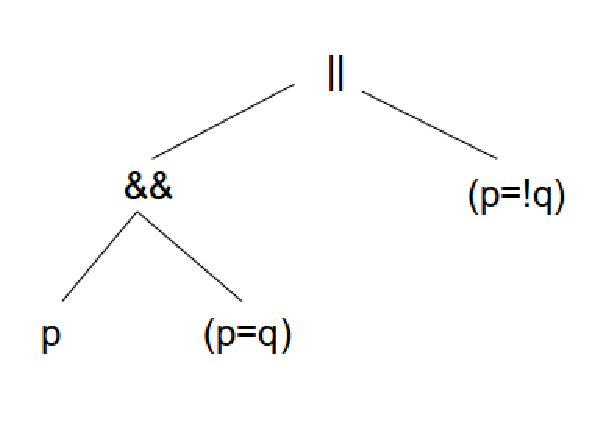
\includegraphics[scale=0.5]{tree.eps} 
\caption{AST for the boolean expression}
\end{figure}


In a first step the left subtree of the AST with the root OR is evaluated:
\begin{equation}
p \quad \&\& \quad (p=q)
\end{equation}
If this subexpression is true then C compiler evaluates the whole expression as true.

But if the subexpression is false the C compiler proceeds with the right subtree of the AST. In this case it evaluates the subexpression:
\begin{equation}
 \quad (p = !q)
\end{equation}
If this subexpression is true the whole expression is evaluated as true, otherwise it's evaluated as false.

\newpage
\subsubsection*{5. Conditional Expression}
\begin{lstlisting}
printf("%i\n", (x < y) ? x : y);
\end{lstlisting}
This statement is equivalent to:
\begin{lstlisting}
int m;
if (x < y)
	m = x;
else 
	m = y;
printf("%i\n", m);
\end{lstlisting}
The tenary expression computes the miniumun of x and y. If x $<$ y holds then the statement following the ? symbol is evaluated, otherwise y is evaluated.

Output is given by:
\begin{lstlisting}
2
\end{lstlisting}
\subsubsection*{6. Bitwise operator}
\paragraph{a)}
To illustrate the bitwise operators we use the integer value x=4.
\begin{equation}
[4]_{10} = [0000 \: 0100 ]_{2}
\end{equation}
The bitwise operation $x<<1$ shifts the bits from left to right by one bit. So after this operation $x$ is stored in the memory as follows:
\begin{equation}
\begin{split}
[0000 \: 1000 ]_{2} = [8]_{10} \\ 
= 0 \cdot 2^7 + 0 \cdot 2^6 + 0 \cdot 2^5 + 0 \cdot 2^4 + 1 \cdot 2^3 + 0 \cdot 2^2 + 0 \cdot 2^1 + 0 \cdot 2^0 \\
= 2^3 = 8
\end{split}
\end{equation}
Because the bases of the binary system are to the power of 2, a shift of one bit position corresponds to a multiplication with two. Analogously, this  holds for the right shift operation.


The bitweise right shift yields:
\begin{equation}
[0000 \: 0010 ]_{2} = [2]_{10} \\ 
\end{equation}
\paragraph{b)}
The following function setbit(x,n) sets the n-th bit to one:
\begin{lstlisting}
#include<stdio.h>
unsigned long setbit(unsigned long x, int n){
        return x | (1UL<<n);
}
main(){
        unsigned long t = 0;
        unsigned long k = setbit(t,2); //0000 => 0100
        printf("%lu\n",k); //4
}
\end{lstlisting}

\subsubsection*{7. Order of Evaluation}
\paragraph{a)}
The statement $f() + g()$ can produce different results for instance with the following function definitions and the variable my\_value:

\begin{lstlisting}
#include<stdio.h>
int f(int *value){ 
        *value = *value * 2; return *value; 
}
int g(int *value){ 
        *value = *value + 1; return *value; 
}
main(){
        int my_value = 2; int res = f(&my_value)+g(&my_value);
        printf("%i\n",res);
}
\end{lstlisting}

If the function $f()$ is called before $g()$ this leads to my\_value=5. But if $g()$ is called before $f()$ then my\_value will be equals to 9.
On my machine I've got the result 9. So on my machine evaluates the function g first.

Briefly speaking: Function with side-effects are vulnerable to such problems.

\paragraph{b)}
This statement below can produce different results if the variable n is a pointer.
\begin{lstlisting}
printf("%i\n", ++n, f(n));
\end{lstlisting}

If we assume that n points to the top of a c-string and the function f(n) just returns the character in c-string at the n-th position then its crucial if the address n is incremented before the function call $f(n)$.

Here's an example:
\begin{lstlisting}
#include<stdio.h>
char f(char *n){
	return *n;
}

main(){
	char c[] = "AB";
	char* n = c;
	printf("letter: %i \t %i\n", ++n ,f(n)); //address 65
	printf("letter: %i \t %i\n", ++n ,f(n)); //address 66
}
\end{lstlisting}
On my machine the function $f(n)$ is called before the address n is incremented.

\subsection*{Part 2: System and Unix}
\subsubsection*{8. Memory Diagrams}
We've the following program:
\begin{lstlisting}
(01) main() {
(02)     int i=8;
(03)     char c1='@', c2='A';
(04)     char s[5]="@A";
(05) }
\end{lstlisting}
According the ASCII table the characters correspond to:
\begin{itemize}[noitemsep]
\item @ = 0x40
\item A = 0x41
\item 8 = 0000 1000 = 0x08
\end{itemize}
\paragraph*{a)}
\quad
\begin{figure}[!htb]
\centering
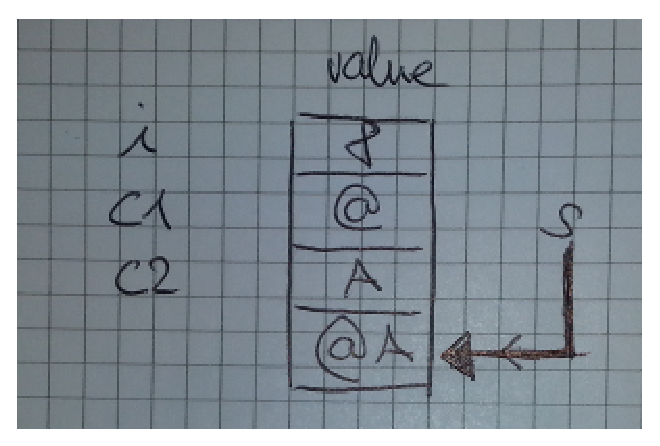
\includegraphics[scale=0.5]{mem_a.eps} 
\end{figure}

\paragraph*{b)}
\quad
\begin{figure}[!htb]
\centering
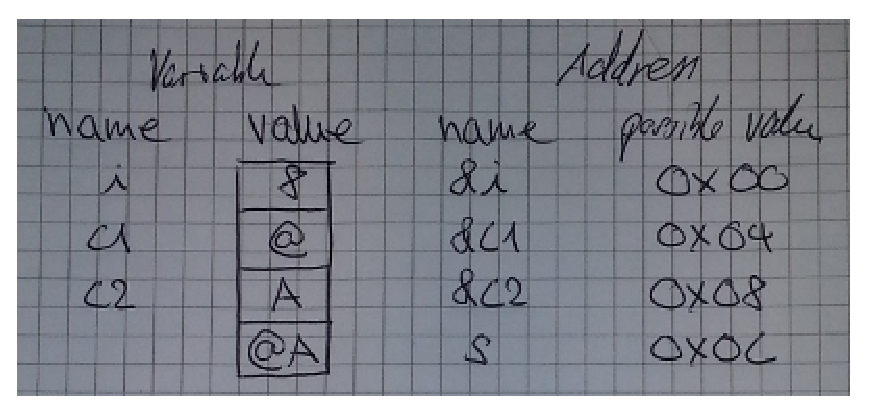
\includegraphics[scale=0.6]{mem_b.eps} 
\end{figure}

\paragraph*{c)}
\quad
\begin{figure}[!htb]
\centering
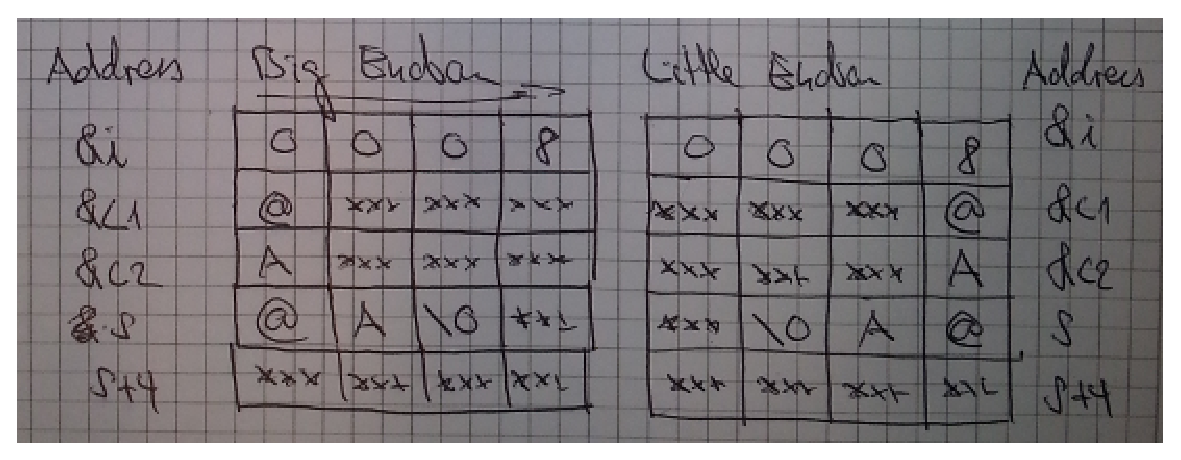
\includegraphics[scale=0.75]{mem_c.eps} 
\end{figure}

\paragraph*{d)}
\quad
\begin{figure}[!htb]
\centering
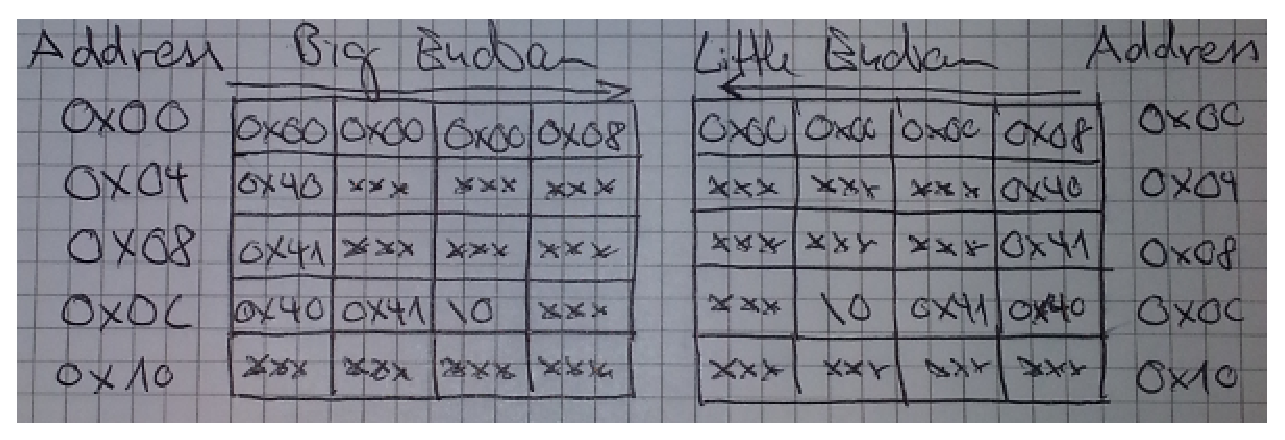
\includegraphics[scale=0.75]{mem_d.eps} 
\end{figure}


\subsubsection*{9. scanf}
\paragraph*{a) A simple program with input errors}
\quad
\begin{lstlisting}
(1) d = scanf("%s %i", str, &i);
\end{lstlisting}
The function call scanf() contains two input fields. It reads two items from the stdin and stores the values in the corresponding addresses str and \&i. The first item is a c-string and the second item is an integer. In this example the values AA and 33 are read from the file Fig9\_input.txt.

The scanf() function returns an integer value indicating the number of items successfully filled. If scanf() fails it rerturns 0 or a negative value. In this example d is equals to 2, because AA ad 33 are two items.

\begin{lstlisting}
(2) d = scanf("%s %i", str, &i);
\end{lstlisting}
The second line reads the next two items from the input file that is 55 and ZZ. The variable d should contain the value 2.

\begin{lstlisting}
(2) d = scanf("%s %i", str, &i);
\end{lstlisting}
And in the third line the values 77 and 99 are read. The variable d is equals to 2.

On my machine I get the following output:
\begin{lstlisting}
./Fig9a < Fig9a_input.txt
----- Fig. 9a: scan/print 3 times a string followed by an integer -----
d=2: s=AA i=33
d=1: s=55 i=33
d=2: s=ZZ i=77

\end{lstlisting}
The results of line 1 and 3 are line with my answers. But I can't really explain why I get a value of 1 in the variable d in the second line. 

The man page of scanf() says:
\begin{quote}
[...]These functions return the number of input items  successfully  matched and assigned, which can be fewer than provided for, or even zero in the event of an early matching failure.[...]
\end{quote}
Maybe it's a reading error.

\paragraph*{b) A simple program}
The following program reads a char, a string and a float value.
\begin{lstlisting}
#define MAX_LENGTH 20
#include<stdio.h>
main(){
        char c; char s[MAX_LENGTH]; float f;
        printf("please enter a char, a string and a float value:\n");
        scanf("%c %s %f",&c,s,&f);
        printf("c=%c \t s=%s \t f=%f\n",c,s,f);
}
\end{lstlisting}
To test this simple program I created an input file with the content:
\begin{lstlisting}
A Alexander 3.14
\end{lstlisting}
The test shows the output:
\begin{lstlisting}
./scanf_program < scanf_program_input.txt 
please enter a char, a string and a float value:
c=A 	 s=Alexander 	 f=3.140000
\end{lstlisting}
\subsubsection*{10. Unix variables}
On my machine the PATH variable is set as follows:
\begin{lstlisting}
/usr/local/sbin:/usr/local/bin:/usr/sbin:/usr/bin:/sbin:/bin:/usr/games:
/usr/local/games:/home/lexruee/projects/cakephp/lib/Cake/Console:
./
\end{lstlisting}
Using the following command I append the current directory to the PATH  variable:
\begin{lstlisting}
PATH=$PATH:./
\end{lstlisting}
As we can see in the last line that the current directory is succesfully appended to the system PATH variable.
\begin{lstlisting}
echo $PATH
/usr/local/sbin:/usr/local/bin:/usr/sbin:/usr/bin:/sbin:/bin:/usr/games:
/usr/local/games:/home/lexruee/projects/cakephp/lib/Cake/Console:
./
\end{lstlisting}


\end{document}
